 \chapter{Магнитное поле в вакууме}

\section{Определение магнитного поля}
\label{sec8.1}

    Оказывается, что если заряд движется, то на него, помимо Кулоновской силы
    \( \vec{F}_\textit{Кул} \), пропорциональной его заряду \( q \), действует
    и другая сила \( F \), пропорциональная и его заряду \( q \) и скорости
    \( v \), с которой он движется, причем \( \vec{F} \perp \vec{v} \), которая
    называется \textit{магнитной}.
    
    \begin{definition}
        Если на точечный заряд \( q \), движущийся в некоторой системе отсчета 
        в области \( V \) с некоторой скоростью \( v \), действует магнитная
        сила, то говорят, что в этой области и \textit{в этой системе отсчета}
        есть \textbf{магнитное поле} \( \vec{B} \), величина и направление
        которого определяется формулой Лоренца:
        \begin{equation}
            \vec{F} = q(\vec{v} \times \vec{B})
            \label{eq8:1}
        \end{equation}
    \end{definition}
    
    \begin{remark}
        Часто формулу Лоренца записывают в обобщенном виде:
        \begin{equation}
            \vec{F} = q\vec{E} + q(\vec{v} \times \vec{B})
            \label{eq8:1a}
        \end{equation}
    \end{remark}
    
    \begin{remark}
        Так как \( \vec{F} \perp \vec{v} \), то поле \( \vec{B} \) работы не
        совершает.
    \end{remark}
   
    \begin{figure}[b!]
        \center
        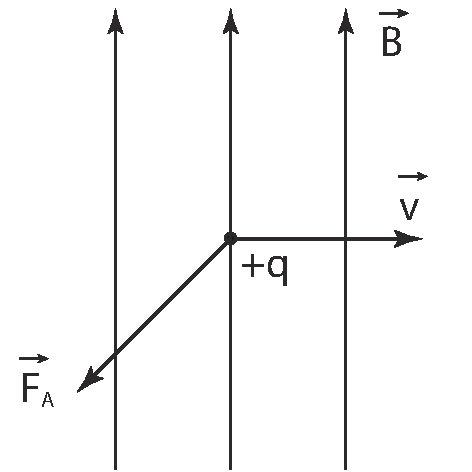
\includegraphics[width=0.3\textwidth]{lec08/magnetic_def.pdf}
        \hfill
        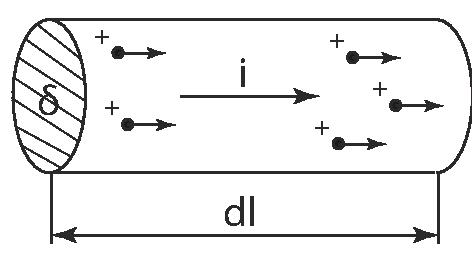
\includegraphics[width=0.3\textwidth]{lec08/conductor.pdf}
        \hfill
        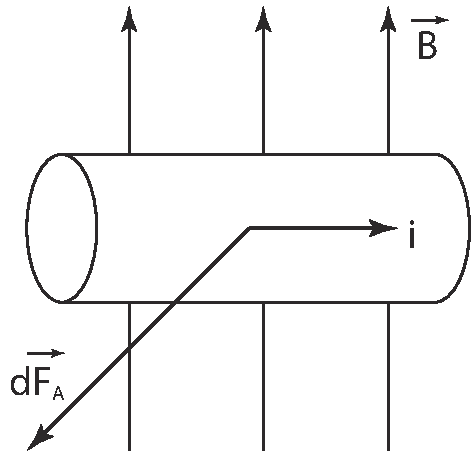
\includegraphics[width=0.3\textwidth]{lec08/conductor_in_mf.pdf}
        \parbox[t]{.3\textwidth}{\caption{К определению магнитного поля}}
        \hfill
        \parbox[t]{.3\textwidth}{\caption{Проводник с током}}
        \hfill
        \parbox[t]{.3\textwidth}{\caption{Действие магнитного поля на проводник
            с током}}
    \end{figure}

\section{Действие магнитного поля на ток (сила Ампера)}

    Рассмотрим проводник с током, помещенный в поле \( \vec{B} \). Вырежем из
    проводника малый элемент \( dV = Sdl \). На каждый заряд в элементе
    действует сила (\ref{eq8:1}). Этот элемент содержит заряд \( dq = e dN \),
    где \( dN = ndV = nSdl \) -- число свободных зарядов в элементе \( dV \),
    \( n \) -- концентрация свободных зарядов.
    
    Таким образом, \( dq = neSdl \). Тогда, в силу (\ref{eq8:1}), на этот
    элемент тока действует сила
    \[
        \vec{dF} = dq(\vec{v} \times \vec{B}) = (ne\vec{v} \times \vec{B})Sdl =
        (\vec{j} \times \vec{B})Sdl.
    \]
    А так как в линейном проводнике \( \vec{dl} \uparrow\uparrow \vec{j} \), а
    \( jS = i \), то
    \begin{equation}
        \vec{dF}_A = i(\vec{dl} \times \vec{B})
        \label{eq8:2}
    \end{equation}
    
    Уравнение (\ref{eq8:2}) определяет силу Ампера.
    
\section{Действие магнитного поля на контур с током. Магнитный момент контура с
    током}
    \begin{figure}[b]
        \center
        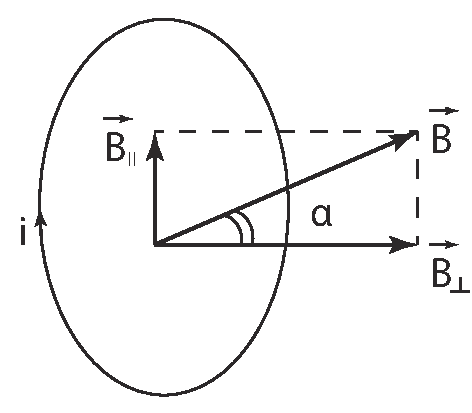
\includegraphics[width=0.3\textwidth]{lec08/contour.pdf}
        \hfill
        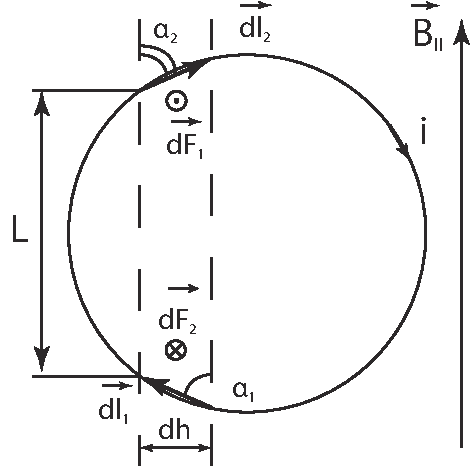
\includegraphics[width=0.3\textwidth]{lec08/calculate_moment.pdf}
        \hfill
        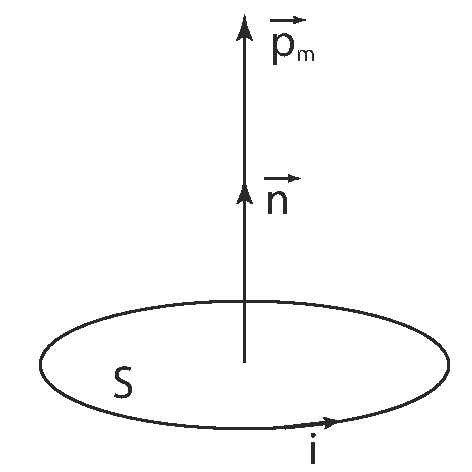
\includegraphics[width=0.3\textwidth]{lec08/magnetic_moment.pdf}
        \parbox[t]{.3\textwidth}{\caption{Контур в магнитном поле}}
        \hfill
        \parbox[t]{.3\textwidth}{\caption{Действие параллельной составляющей
            магнитного поля на контур}}
        \hfill
        \parbox[t]{.3\textwidth}{\caption{Магнитный момент контура}}
    \end{figure}

    Пусть плоский контур с током \( i \) находится в однородном поле
    \( \vec{B} \), направленным под углом \( \alpha \) к нормали к плоскости
    контура. Тогда поле \( \vec{B} \) можно разложить на две составляющие:
    \[
        \vec{B} = \vec{B}_{\perp} + \vec{B}_{\|},
    \]
    где \( B_{\|} = B\sin\alpha \) -- параллельная плоскости компонента, а
    \( B_{\perp} = B\cos\alpha \) -- перпендикулярная ей компонента.
    
    Компонента \( \vec{B}_{\perp} \) либо сжимает контур, либо растягивает его:
    \[
        \vec{dF}_A = i(\vec{dl} \times \vec{B}_{\perp}).
    \]
    
    Рассмотрим влияние компоненты \( \vec{B}_{\|} \). Вырежем из контура с током
    узкую полоску длины \( L \) и ширины \( dh \), тогда \( \vec{dl}_1 \) и 
    \( \vec{dl}_2 \) есть вырезанные элементы тока, а площадь полоски
    \( dS = Ldh \).
    
    На вырезанные элементы будут действовать силы:
    \[
        \left\{
        \begin{array}{c}
            \vec{dF}_1 = i(\vec{dl}_1 \times \vec{B}_{\|}), \\
            \vec{dF}_2 = i(\vec{dl}_2 \times \vec{B}_{\|});
        \end{array}
        \right. \\
    \]
    \[
        \left\{
        \begin{array}{c}
            \vec{dF}_1 = iB_{\|}dl_1\sin\alpha_1 = iB_{\|}dh, \\
            \vec{dF}_2 = iB_{\|}dl_2\sin\alpha_2 = iB_{\|}dh.
        \end{array}
        \right. \\
    \]

    Таким образом, \( dF_1 = dF_2 \), следовательно они образуют пару сил,
    момент на полоску которой:
    \[
        dM = LdF = (Ldh)iB_{\|} = iB_{\|}dS.
    \]
    
    Интегрируя по всем полоскам получим момент сил Ампера на контур с током:
    \begin{equation}
        M = iB_{\|}S.
        \label{eq8:2a}
    \end{equation}
    
    \begin{definition}
        Пусть по плоскому контуру площади \( S \) идет ток \( i \). Тогда
        векторная величина
        \begin{equation}
            \vec{p}_m = i\vec{n}S = i\vec{S}
            \label{eq8:2b}
        \end{equation}
        называется \textbf{магнитным моментом контура}, а сам контур --
        \textbf{магнитным диполем}.
    
        Вектор \( \vec{S} = \vec{n}S \) образует правый винт с направлением
        движения положительных зарядов (со стрелкой тока) в контуре.
    \end{definition}
    
    Тогда формулу (\ref{eq8:2a}) можно записать так:
    \[
        M = p_mB_{\|} = p_mB\sin\alpha
    \]
    или в векторном виде:
    \begin{equation}
        \vec{M} = \vec{p}_m \times \vec{B}
        \label{eq8:2c}
    \end{equation}
    
    Момент сил, действующий на контур с током, (\ref{eq8:2c}) стремится
    повернуть контур так, чтобы магнитный момент \( \vec{p}_m \) стал параллелен
    линияям поля \( \vec{B} \). Такое положение называется \textit{устойчивой
    ориентацией}.
    
    Работа поворота контура с током на угол \( d\alpha \)
    \[
        dA = Md\alpha.
    \]
    Тогда, для энергии контура в поле \( \vec{B} \)
    \[
        W = A = \int Md\alpha = \int p_mB\sin\alpha d\alpha = -p_mB\cos\alpha +
        C
    \]
    Полагая, что при \( \alpha = 90^{\circ} \) \( W = 0 \), получим, что
    \( C = 0 \).
    
    Тогда энергия контура с током:
    \begin{equation}
        W = -p_mB\cos\alpha = -\vec{p}_m \cdot \vec{B}
        \label{eq8:2d}
    \end{equation}
    
    Так как \( \vec{F} = -\nabla W \), то на магнитный диполь действует сила
    \( \vec{F} = \nabla(\vec{p}_m\cdot\vec{B}) \), а при \( p_m = \const \) сила
    будет
    \[
        \vec{F} = (\vec{p}\cdot\nabla)\vec{B}.
    \]
    
    Если поле \( \vec{B} \) имеет только \( x \)-компоненту, то есть
    \( \vec{B} = \{B_x, 0 , 0\} \), то сила
    \[
        \vec{F}_x = p_m\frac{\partial \vec{B}}{\partial x}
    \]
    будет ориентировать диполь в устойчивую ориентацию вдоль оси \( Ox \) и
    втягивать его в область более сильного поля.
    
\section{Магнитное поле движущегося заряда. Закон Био-Савара}

    Мы рассмотрели действие магнитного поля на токи и заряды. Рассмотрим вопрос
    о порождении магнитного поля.
    
    Опыт показывает, что оно создается движущимися зарядами или токами.
    Экспериментально установлено, что если точечный заряд \( q \) движется со
    скоростью \( \vec{v} \), то он порождает в окружающем пространстве магнитное
    поле
    \begin{equation}
        \vec{B} = k_mq\frac{\vec{v}\times\vec{r}}{r^3}
        \label{eq8:3}
    \end{equation}
    Формула (\ref{eq8:3}) называется законом Био-Савара.
    \begin{figure}[!b]
        \center
        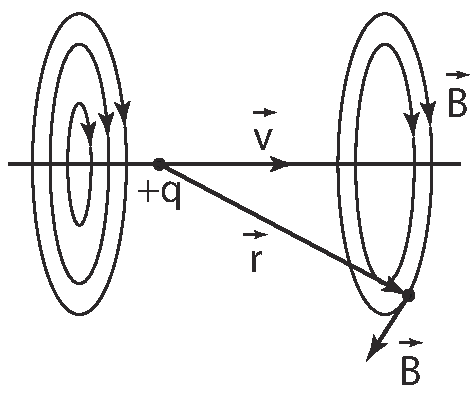
\includegraphics[width=.47\textwidth]{lec08/Bio_Savar.pdf}
        \hfill
        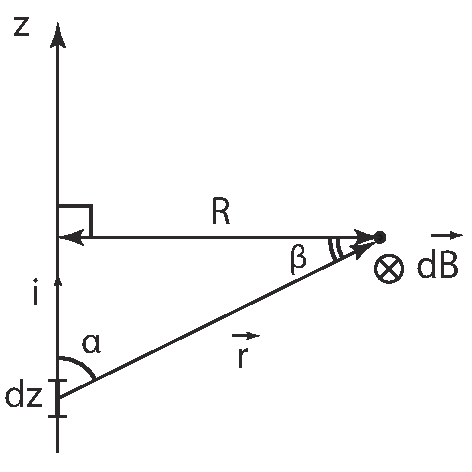
\includegraphics[width=.47\textwidth]{lec08/Bio_Savar_i.pdf}
        \parbox[t]{.47\textwidth}{\caption{Магнитное поле заряда, движущегося
            равномерно и прямолинейно}}
        \hfill
        \parbox[t]{.47\textwidth}{\caption{Расчёт магнитного поля прямого тока
            при помощи закона Био-Савара}}
    \end{figure}
    В системе СИ
    \[
        k_m = \frac{1}{4\pi\eps_0 c^2}.
    \]
    Величина
    \[
        \frac{1}{\eps_0 c^2} = \mu_0 =
        4\pi \cdot 10^{-7} \frac{\text{Гн}}{\text{м}}
    \]
    называется \textit{магнитной постоянной}.
    
    Тогда закон Био-Савара в СИ принимает вид
    \begin{equation}
        \vec{B} = \frac{\mu_0}{4\pi} q \frac{\vec{v}\times\vec{r}}{r^3}
        \label{eq8:4}
    \end{equation}

\section{Магнитное поле тока}
    Вычислим из (\ref{eq8:4}) магнитное поле малого элемента проводника
    \( \vec{dl} \). В объеме \( dV = Sdl \) находится свободный заряд
    \( dq = (ndV)e = neSdl \). Этот заряд движется со скоростью
    \( \vec{v}_{\textit{др}} \), следовательно, в силу (\ref{eq8:4}) он
    порождает поле:
    \[
        \vec{dB} = \frac{\mu_0}{4\pi}neSdl\frac{\vec{v}\times\vec{r}}{r^3} =
        \frac{\mu_0}{4\pi} \left(\frac{ne\vec{v}\times\vec{r}}{r^3}\right)Sdl.
    \]
    
    А так как \( ne\vec{v} = \vec{j}, \, jS = i, \,
    \vec{j} \uparrow\uparrow \vec{dl} \), то
    \begin{equation}
        \vec{dB} = \frac{\mu_0}{4\pi} i \frac{\vec{dl}\times\vec{r}}{r^3}.
        \label{eq8:5}
    \end{equation}
    
    Поле \( \vec{B} \) подчиняется принципу суперпозиции:
    \[
        \vec{B} = \sum \Delta\vec{B}_k,
    \]
    где \( \vec{B} \) -- поле всего провода, а \( \Delta\vec{B}_k \) -- поле
    отдельных элементов проводника.
    
    Тогда какой-либо контур с током \( i \) создаст поле:
    \begin{equation}
        \vec{B} = \frac{\mu_0}{4\pi} i \oint\limits_C \frac{\vec{dl}\times
        \vec{r}}{r^3} 
        \label{eq8:6}
    \end{equation}
    
    \begin{example}
        Вычислить поле \( \vec{B} \) прямого бесконечного провода с током
        \( i \).
    \end{example}
    
    \begin{solution}
        Каждый элемент \( \vec{dl} \) провода создает поле
        \[
            \vec{dB} = k\frac{\vec{dl}\times\vec{r}}{r^3}.
        \]
        \[
            dB = k\frac{dz r’}{r'^3}\sin\beta = k\frac{dz\cos\alpha}{r'^2} = 
            k\frac{dz\cos\alpha}{ \frac{r^2}{\cos^2\alpha} }.
        \]
        А так как \( z = r\tg\alpha \), то
        \[
            dz = \frac{r}{\cos^2\alpha}d\alpha.
        \]
        Тогда
        \[ dB = k\frac{\cos\alpha}{r}d\alpha, \]
        а поле всего проводника
        \[
            B = \frac{k}{r} \int\limits_{ -\frac{\pi}{2} }^{ \frac{\pi}{2} }
            \cos\alpha d\alpha = \frac{2k}{r} = \frac{\mu_0}{2\pi r}i.
        \]
        
        В цилиндрических кординатах:
        \[
            \vec{B}(\rho, \varphi, z) =
            \frac{\mu_0 i}{2\pi}\left\{0, \frac{1}{\rho}, 0\right\}.
        \]
        
        В декартовых:
        \[
            \vec{B}(x, y, z) = \frac{\mu_0 i}{2\pi r^2}\{ -y, x, 0 \}.
        \]
    \end{solution}
    
\section{Взаимодействие параллельных токов. Определение Ампера}

    Пусть по двум бесконечно длинным тонким прямым проводам в вакууме текут токи
    \( i_1 \) и \( i_2 \). Тогда ток \( i_1 \) создает на линии тока \( i_2 \)
    поле
    \[
        B_1 = \frac{\mu_0 i_1}{2\pi a}.
    \]
    Следовательно, на элемент \( \vec{dl}_2 \) с током \( i_2 \) действует сила
    Ампера
    \[
        \vec{dF}_{21} = i_2(\vec{dl}_2\times\vec{B}_1),
    \]
    направленная к другому проводнику. Так как \( \vec{B}_1 \perp \vec{dl}_2 \),
    то
    \[
        dF_{21} = \frac{\mu_0 i_1i_2}{2\pi a}dl_2.
    \]
    Следовательно, погонная сила, дествующая на провод \( i_2 \) равна
    \begin{equation}
        F_{20} = \frac{dF_{21}}{dl_2} = \frac{\mu_0 i_1 i_2}{2\pi a}
        \label{eq8:7}
    \end{equation}
    Очевидно, что и на провод с током \( i_1 \) действует равная
    \( \vec{F}_{20} \) по модулю погонная сила, только направленная в другую
    сторону: \( \vec{F}_{10} = - \vec{F}_{20} \).
    
    \textbf{Два параллельных проводника с токами, текущими в одну сторону,
    притягиваются, а с токами, текущими в противоположные стороны, --
    отталкиваются}
    
    Положим в (\ref{eq8:7}): \( a = 1 \)м, \( i_1 = i_2 = 1\)ед. тока. Тогда
    \[
        F_{10} = F_{20} = \frac{\mu_0}{2\pi} =
        2 \cdot 10^{-7} \left(\frac{\text{Н}}{\text{м}}\right).
    \]
    
    \begin{definition}
        1 \textbf{Ампер} -- это ток, который, проходя по каждому из двух тонких
        прямых параллельных проводов, удалённых друг от друга на 1 м в вакууме,
        создает между ними силу притяжения (или отталкивания)
        \( F_0 = 2 \cdot 10^{-7} \)Н на каждый метр длины.
    \end{definition}
    
    \begin{figure}[b!]
        \center
        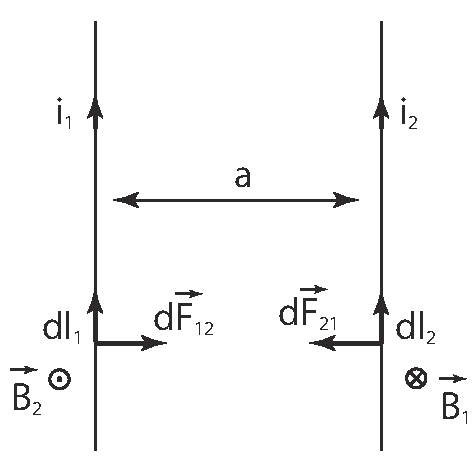
\includegraphics[width=.47\textwidth]{lec08/current_interaction.pdf}
        \hfill
        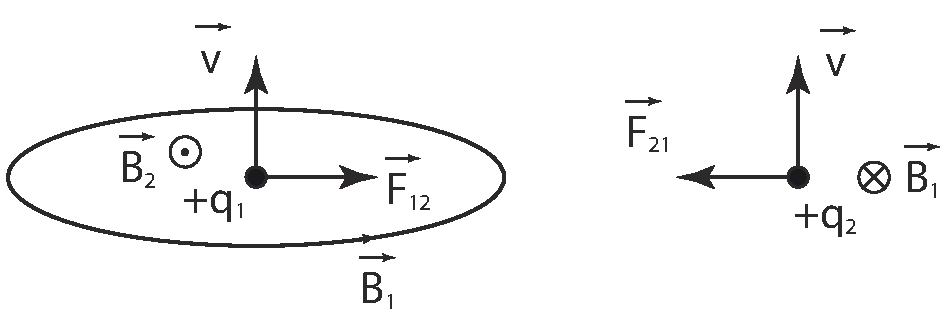
\includegraphics[width=.47\textwidth]{lec08/charge_interaction.pdf}
        \parbox[t]{.47\textwidth}{\caption{Взаимодействие токов}}
        \hfill
        \parbox[t]{.47\textwidth}{\caption{Магнитное взаимодействие зарядов}}
    \end{figure}

\section{Взаимодействие движущихся зарядов}
    Пусть два заряда \( q_1 \) и \( q_2 \) движутся с одинаковыми скоростями
    параллельными курсами. Тогда один заряд создает поле
    \[
        \vec{B}_1 = \frac{\mu_0}{4\pi} q_1 \frac{\vec{v}\times\vec{r}}{r^3}.
    \]
    Следовательно, на \( q_2 \) действует сила Лоренца
    \[
        \vec{F}_{21} = q_2(\vec{v}\times\vec{B}_1) =
        \frac{\mu_0}{4\pi} q_1q_2 \frac{1}{r^3}
        (\vec{v}\times(\vec{v}\times\vec{r}).
    \]
    А так как \( \vec{v} \perp \vec{r} \), то по модулю:
    \[
        F_{21} = \frac{\mu_0}{4\pi}\frac{q_1q_2}{r^2}v^2.
    \]    
    Аналогично, \( \vec{F}_{12} = -\vec{F}_{21} \).
    
    Таким образом, два одноимённых заряда, летящие параллельными курсами,
    магнитно притягиваются. А так как \( \mu_0 = \frac{1}{\eps_0 c^2} \), то
    \[
        F_{12} = F_{21} = F_{\textit{маг}} =
        \frac{q_1q_2}{4\pi\eps_0 r^2} \left(\frac{v^2}{c^2}\right)
    \]
    Также они отталкиваются кулоновской силой
    \[
        F_{\textit{кул}} = \frac{q_1q_2}{4\pi\eps_0 r^2}.
    \]
    Отношение сил будет
    \[
        \frac{F_{\textit{маг}}}{F_{\textit{кул}}} = \frac{v^2}{c^2},
    \]
    а так как обычно \( v \ll c \), то \( F_\textit{маг} \ll F_\textit{кул} \).
    Это приводит к развалу электронных пучков: так, при 
    \( v \approx 0,1 \frac{\text{мм}}{\text{с}} =
    10^{-4} \frac{\text{м}}{\text{с}} \)
    \[
        \frac{F_{\textit{маг}}}{F_{\textit{кул}}} = \frac{v^2}{c^2} =
        \frac{10^{-8}}{9 \times 10^{16}} = 10^{-25}.
    \]
    
    Однако, два параллельных тока притягиваются, так как провода в высшей
    степени электронейтральны и \( F_\textit{кул} = 0 \).
    
\section{Поток поля \textbf{B}}
    Поток поля \( \vec{B} \) через поверхность \( S \)
    \[
        \Phi = \iint\limits_S \vec{B}\cdot\vec{dS} (\text{Вб [Вебер]}).
    \]
    Если поверхность \( S \) замкнута, то
    \[
        \Phi = \oiint\limits_S \vec{B}\cdot\vec{dS}.
    \]
    
    Из факта отсутствия магнитных зарядов следует, что поле \( \vec{B} \) не
    имеет источников: его линии либо замкнуты, либо бесконечны. Это означает,
    что каждая линия поля \( \vec{B} \) пересекает поверхность \( S \) четное
    число раз.
    \[
        \Phi = \oiint\limits_S \vec{B}\cdot\vec{dS} = 0.
    \]
    А по теореме Остроградского:
    \[
        \oiint\limits_S \vec{B}\cdot\vec{dS} = \iiint\limits_V \div\vec{B}dV,
    \]
    \[
        \div\vec{B} = 0.
    \]
     Так как \( \div\vec{B} = 0 \), то поле \( \vec{B} \) соленоидально.
     
\section{Теорема о циркуляции поля \textbf{B}}
    \begin{theorem}
        Пусть токи \( i_1, i_2, \ldots, i_n \) охватываются некоторым контуром
        \( C \). Тогда цикуляция поля \( \vec{B} \) по контуру \( C \) равна
        алгебраической сумме токов, охватываемых этим контуром, помноженной на
        \( \mu_0 \):
        \begin{equation}
            \oint\limits_C \vec{B}\cdot\vec{dl} = \mu_0 (\sum \pm i_k)_C
            \label{eq8:n1}
        \end{equation}
    \end{theorem}

    \begin{figure}[!b]
        \center
        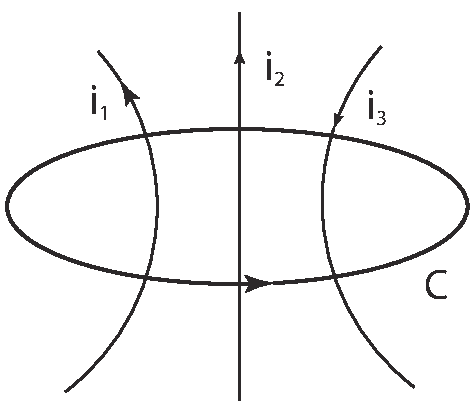
\includegraphics[width=0.3\textwidth]{lec08/circulation_B.pdf} 
        \caption{К теореме о циркуляции}
        \label{fig:circulation_B}
    \end{figure}
    
    \begin{remark}
        Ток \( i_k \) считается положительным, если его стрелка образует правый
        винт с направлением обхода контура \( C \). Например,
        на рисунке~\ref{fig:circulation_B}
        \[
            i_1, i_2 > 0; \, i_3 < 0,
        \]
        и теорема о циркуляции поля \( \vec{B} \) принимает вид
        \[
            \oint\limits_C \vec{B}\cdot\vec{dl} = \mu_0 (i_1 + i_2 - i_3)
        \]
    \end{remark}
    
    \begin{proof}
    Для случая произвольных токов доказательство слишком громоздко. Поэтому
    докажем теорему для случая прямых токов. Пусть контур \( C \) охватывает
    только один прямой ток \( i \). Распишем циркуляцию поля \( \vec{B} \) в
    цилиндрических координатах:
    \begin{align*}
        \Gamma = & \oint\limits_C \vec{B}\cdot\vec{dl} =
        \oint\limits_C \sum B_iH_idq_i =
        \oint\limits_C \frac{\mu_0 i}{2\pi}\frac{1}{r}rd\varphi = \\
        = & \oint\limits_C \frac{\mu_0 i}{2\pi} d\varphi =
        \frac{\mu_0 i}{2\pi} \oint\limits_0^{2\pi}d\varphi = \mu_0 i.
    \end{align*}
    
    Пусть контур \( C \) охватывает несколько токов. Тогда, в силу принципа
    суперпозиции, получаем
    \[
        \oint\limits_C \vec{B}\cdot\vec{dl} = \sum\limits_k
        \underbrace{ \oint\limits_C \vec{B}_k\cdot\vec{dl} }_{\mu_0 i_k} =
        \mu_0 (\sum i_k)_C.
    \]
    \end{proof}
    
    Пусть ток распределен в пространстве непрерывно с плотностью \( \vec{j} \),
    тогда, так как
    \[
        i = \iint\limits_S \vec{j}\cdot\vec{dS},
    \]
    \[
        \oint\limits_C \vec{B}\cdot\vec{dl} =
        \mu_0 \iint\limits_S \vec{j}\cdot\vec{dS}.
    \]
    По теореме Стокса
    \[
        \oint\limits_C \vec{B}\cdot\vec{dl} =
        \iint\limits_S \rot\vec{B}\cdot\vec{dS}.
    \]
    
    Так как поверхность \( S \) -- произвольна, то
    \begin{equation}
        \rot\vec{B} = \mu_0 \vec{j}
        \label{eq8:n2}
    \end{equation}
    Уравнение (\ref{eq8:n2}) -- это дифференциальная форма теоремы о циркуляции
    поля \( \vec{B} \) (\ref{eq8:n1}).
    
\section{Основные уравнения магнитостатики для вакуума}

    \begin{tabular}[ht]{|c|c|c|c|} \hline
    Название & \(\int\)-форма & d-форма & Cмысл \\ \hline
    & & & \\
    %-----------------------------------------------------------------
    Поток поля \( \vec{B} \) & \(\oiint\limits_S \vec{B}\cdot\vec{dS} = 0 \)
        & \( \div\vec{B} = 0 \) & поле \(\vec{B}\) не имеет источников \\
    %-----------------------------------------------------------------
    Теорема о циркуляции & \(\int\limits_C \vec{B}\cdot\vec{dl} = \mu_0 i_C \)
        & \( \rot\vec{B} = \mu_0\vec{j} \) & поле \(\vec{B}\) порождается током
        \\
    %-----------------------------------------------------------------
    & & & \\ \hline
    \end{tabular}
    
\section{Примеры использования теоремы о циркуляции}

    Теорема о циркуляции (\ref{eq8:n1}) в общем случае не позволяет вычислить
    поле \( \vec{B} \) от заданной системы токов, так как значение интеграла
    \[
        \oint\limits_C \vec{B}\cdot\vec{dl}
    \]
    не определяет \( \vec{B} (x, y, z) \).
    
    Однако, для некоторых симметричных конфигураций токов она служит эффективным
    инструментом расчета поля \( \vec{B} \).
    
    \begin{example}
        Вычислить распределение поля \( \vec{B}(r) \) толстого провода радиуса
        \( R \) с током \( i \), равномерно распределенного по сечению.
    \end{example}
    
    \begin{figure}[!t]
        \center
        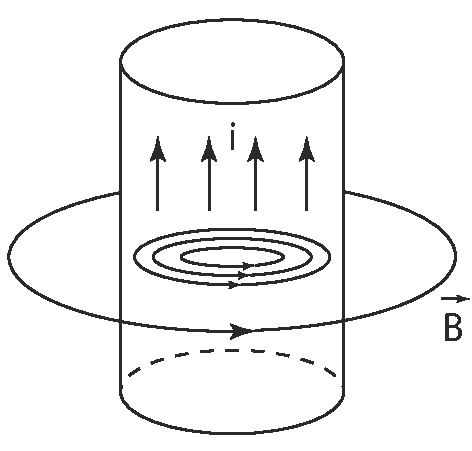
\includegraphics[width=.47\textwidth]{lec08/conductor_B.pdf}
        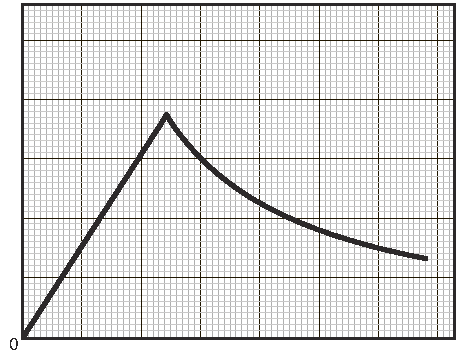
\includegraphics[width=.47\textwidth]{lec08/conductor_B_plot.pdf}
        \parbox[t]{.47\textwidth}{\caption{Поле в толстом проводнике}}
        \parbox[t]{.47\textwidth}{\caption{Зависимость величины поля от
            расстояния о центра проводника}
            \label{fig:B_in_fat_wire}}
    \end{figure}

    \begin{solution}
        \begin{enumerate}
            \item \( r > R \). Охватим весь провод круговым контуром радиуса
                \( r > R \). Тогда
                \[
                    \oint\limits_{2\pi r} \vec{B}_{ex}\cdot\vec{dl} = \mu_0 i.
                \]
                А так как вдоль контуре \( B = const \), то 
                \( \vec{B} \uparrow\uparrow \vec{dl} \) и
                \[
                    \oint\limits_{2\pi r}\vec{B}_{ex}\cdot\vec{dl} = 2\pi B_{ex}r.
                \]
                Отсюда, при \( r > R \):
                \[
                    B_{ex} = \frac{\mu_0 i}{2\pi r}.
                \]
                
            \item \( r < R \). Охватим внутреннюю часть провода круговым
            контуром радиуса \( r < R \). Тогда мы вырезаем ток
            \[
                i_r = j \pi r^2 = \frac{i}{\pi R^2}\pi r^2 = i\frac{r^2}{R^2}.
            \]
            Тогда
            \[
                \oint\limits_{2\pi r} \vec{B}_{in}\cdot\vec{dl} =
                2\pi B_{in} r = \mu_0 i \frac{r^2}{R^2},
            \]
            \[
                B_{in}(r) = \frac{\mu_0 i}{2\pi R^2}r.
            \]
        \end{enumerate}
        
        График этой зависимости представлен на рисунке~\ref{fig:B_in_fat_wire}
    \end{solution}
    
    \begin{example}
        Вычислить распределение поля \( \vec{B}(r) \) коаксиальной линии
        радиусов \( R_1 \) и \( R_2 \), по которой идет ток \( i \).
    \end{example}
    
        \begin{figure}[t!]
            \center
            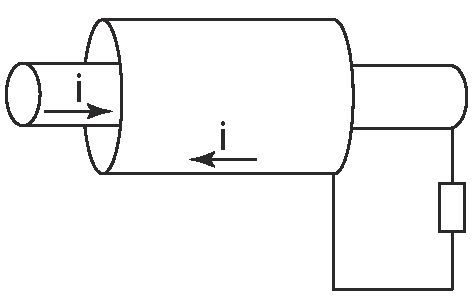
\includegraphics[width=0.3\textwidth]{lec08/coaxial_line.pdf}
            \hfill
            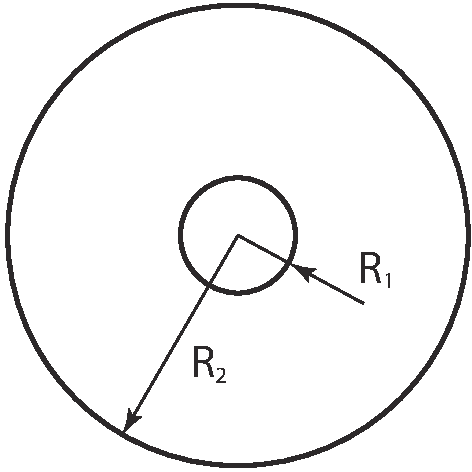
\includegraphics[width=0.3\textwidth]{lec08/coaxial_end.pdf}
            \hfill
            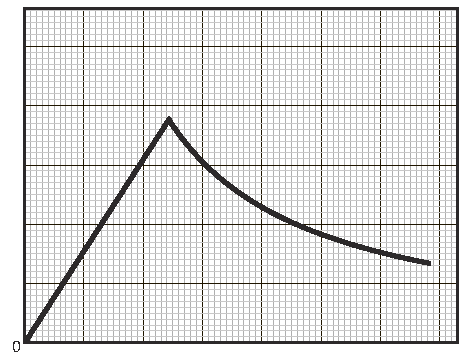
\includegraphics[width=0.3\textwidth]{lec08/coaxial_plot.pdf}
            \parbox[t]{.3\textwidth}{\caption{Коаксиальная линия}}
            \hfill
            \parbox[t]{.3\textwidth}{\caption{Вид сбоку}}
            \hfill
            \parbox[t]{.3\textwidth}{\caption{Зависимость поля от расстояния от
                оси}}
        \end{figure}

    \begin{solution}
        Рассуждая аналогично предыдущему примеру, получим следующее
        распределение поля \( \vec{B} \):
        \[
            B(r) = \left\{
            \begin{array}{l l}
                \frac{\mu_0 i}{2\pi R_1^2}r & \text{при } r < R_1 \\
                \frac{\mu_0 i}{2\pi r} & \text{при } R_1 < r < R_2 \\
                0 & \text{при } R_2 < r
            \end{array}
            \right.
        \]
    \end{solution}
    
    \begin{definition}
        \textbf{Соленоид} -- это длинный цилиндрический каркас радиуса \( R \),
        длины \( l \gg R \), на который уложена плотная однослойная обмотка.
    \end{definition}

    \begin{example}
        Найти поле \( \vec{B} \) в соленоиде длины \( l \), имеющего \( N \)
        витков, и по которому идет ток \( i \).
    \end{example}
    
    
    \begin{figure}[b!]
        \center
        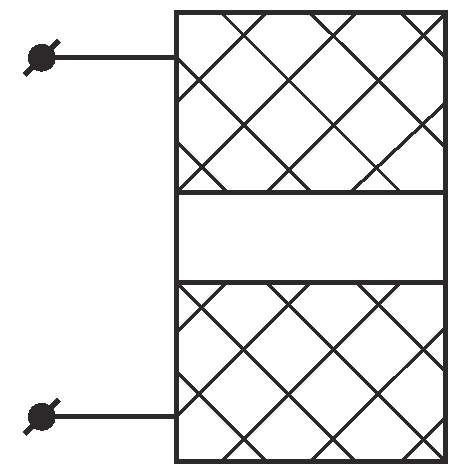
\includegraphics[width=0.3\textwidth]{lec08/fat_solenoid.pdf}
        \hfill
        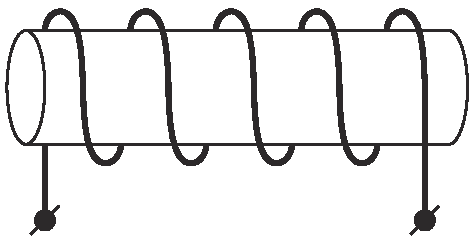
\includegraphics[width=0.3\textwidth]{lec08/loose_solenoid.pdf}
        \hfill
        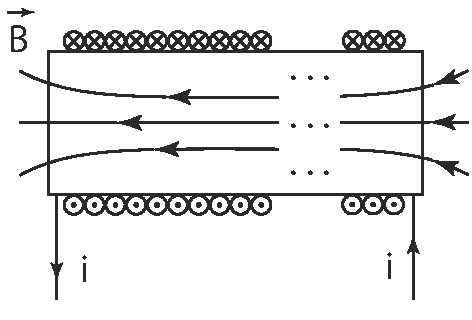
\includegraphics[width=0.3\textwidth]{lec08/solenoid.pdf}
        \parbox[t]{.3\textwidth}{\caption{Слишком толсто для соленоида}}
        \hfill
        \parbox[t]{.3\textwidth}{\caption{Слишком редко для соленоида}}
        \hfill
        \parbox[t]{.3\textwidth}{\caption{Соленоид}}
    \end{figure}
    
    \begin{solution}
        Если соленоид очень длинный (\( l \rightarrow \infty \) или соленоид
        замкнут в тор), то вне соленоида поле \( B_{ex} = 0 \). Окружим стенку
        соленоида узким контуром \( C \) и применим теорему о циркуляции поля
        \( \vec{B} \):
        \[
            \oint\limits_C \vec{B}\cdot\vec{dl} =
            \underbrace{B_{ex}l}_{0} + B_{in}l = \mu_0 (Ni)_C
        \]
        Тогда поле в соленоиде:
        \begin{equation}
            B = \mu_0 \frac{N}{l}i = \mu_0 ni,
            \label{eq8:n3}
        \end{equation}
        где
        \[
            n = \frac{N}{l}
        \]
        плотность витков обмотки.
    \end{solution}
    
\section{Эффект Холла}
    
    В 1880 году Холл открыл следующий эффект: если прямоугольную пластину
    поместить в поле \( \vec{B} \), а перпендикулярно двум другим граням
    пропустить ток \( i \) с плотностью \( j \), то на третьей паре граней
    появится напряжение \( U \ne 0 \), причем \( U \sim B \) и \( U \sim j \).
    
    \textit{картинка} % напиши словами, ок?
    
    Разделение зарядов происходит до тех пор, пока появляющееся в пластине поле
    \( E = \frac{U}{d} \) не будет препятствовать этому, то есть до того, как
    уравняются силы Лоренца и силы Кулона:
    \[
        F_{\textit{Л}} = F_{\textit{Кул}}, \, evB = eE = e\frac{U}{d}.
    \]
    Следовательно, конечное напряжение \( U = Bvd \). А так как \( j = nev \),
    то:
    \begin{equation}
        U = \frac{1}{ne}Bjd
        \label{eq8:n4}
    \end{equation}
    Видно, что \( U \sim jB \). Коэффициент
    \[
        H = \frac{1}{ne}
    \]
    получил название коэффициента (или постоянной) Холла.
    
    Эффект Холла позволяет не только определить концентрацию свободных зарядов
    \( n \), но и знак носителя \( \mp e \) по формуле (\ref{eq8:n4}), где все
    величины (\( U, B, j, d \)) измеряемы. Если \( q = -e \), то при том же
    направлении тока \( i \) полярность \( U \) изменится: 
    % “:” т.к. картинка

    \begin{remark}
        Эффект Холла в металлах очень слаб, так как концентрация свободных
        зарядов в них
        \[
            n \sim 10^{29} \frac{\text{шт}}{\text{м}^3}.
        \]
        Пусть \( d = 0,1 \)м, \( B = 0,1 \)Тл, \( j = 1 \text{А}/\text{мм}^2 \),
        \( e \sim 10^{-19} \)Кл. Тогда
        \[
            U = \frac{1}{ne}Bjd =
            \frac{10^{19}}{10^{29}}10^6 \cdot 10^{-1} \cdot 10^{-3} =
            10^{-8} \text{В} = 0,01 \text{мкВ}.
        \]
    
        Однако, в полупроводниках
        \[
            n \sim 10^{16}-10^{19} \frac{\text{шт}}{\text{м}^3},
        \]
        поэтому эффект Холла в них очень силен.
    \end{remark}
